%----------------------------------------------------------------------------
%	PACKAGES AND OTHER DOCUMENT CONFIGURATIONS
%----------------------------------------------------------------------------

\documentclass[idxtotoc,hyperref,openany]{labbook}

\usepackage[ 
  backref=page,
  pdfpagelabels=true,
  plainpages=false,
  colorlinks=true,
  bookmarks=true,
  pdfview=FitB]{hyperref}
  
\usepackage{booktabs}
\usepackage{float}
\usepackage{graphicx}
\usepackage{lipsum}
\usepackage{siunitx}

\graphicspath{Figures/}

\newcommand{\HRule}{\rule{\linewidth}{0.5mm}}
\setlength\parindent{0pt}
\setlength{\parskip}{\baselineskip}

%----------------------------------------------------------------------------
%	DEFINITION OF EXPERIMENTS
%----------------------------------------------------------------------------

\newexperiment{PPDr}{PPD Repair After PaCE-2022}

%----------------------------------------------------------------------------

\begin{document}

%----------------------------------------------------------------------------
%	TITLE PAGE
%----------------------------------------------------------------------------

\frontmatter % Use Roman numerals for page numbers
\title{
\begin{center}
\HRule \\[0.4cm]
{\Huge \bfseries Laboratory Journal}\\[0.4cm]
\HRule \\[1.5cm]
\end{center}
}
\author{\Huge Jessica Girdwood \\ \\ \LARGE jessgirdwood@protonmail.com \\[2cm]}
\date{Beginning 20\textsuperscript{th} March 2023}
\maketitle

\tableofcontents

\mainmatter

%----------------------------------------------------------------------------
%	LAB BOOK CONTENTS
%----------------------------------------------------------------------------

\labday{20 March 2023}

\experiment{PPDr}

PPD is no longer functional after returning from a campaign in northern Finland. There are no useful images on the screen. When the trigger threshold is lowered to 10, and the trigger PMT voltage is raised above 20, there are noise triggers.

PPD was removed from its pelicase, removing and breaking the seal of the 4 bolts. The inlet heaters were disconnected, and the pump was removed. The arduino was reprogrammed to not trigger the relays. PPD was suspended above  the pelicase on two poles. The grounding point was replaced and connected to the mains socket, the mains cable was also replaced with an English plug.

\labday{21 March 2023}

\experiment{PPDr}

When the output of the trigger PMT was observed with a scope, the signal looked extremely noisy, and repeated at around \SI{5.6}{\kilo\hertz}. Figure \ref{fig:PPDScopeNoise} shows this. I was unable to determine as to whether this was the laser or the PMT, however the laser was visibly damaged so this was the suspected cause at this stage.

\begin{figure}[H]
\begin{center}
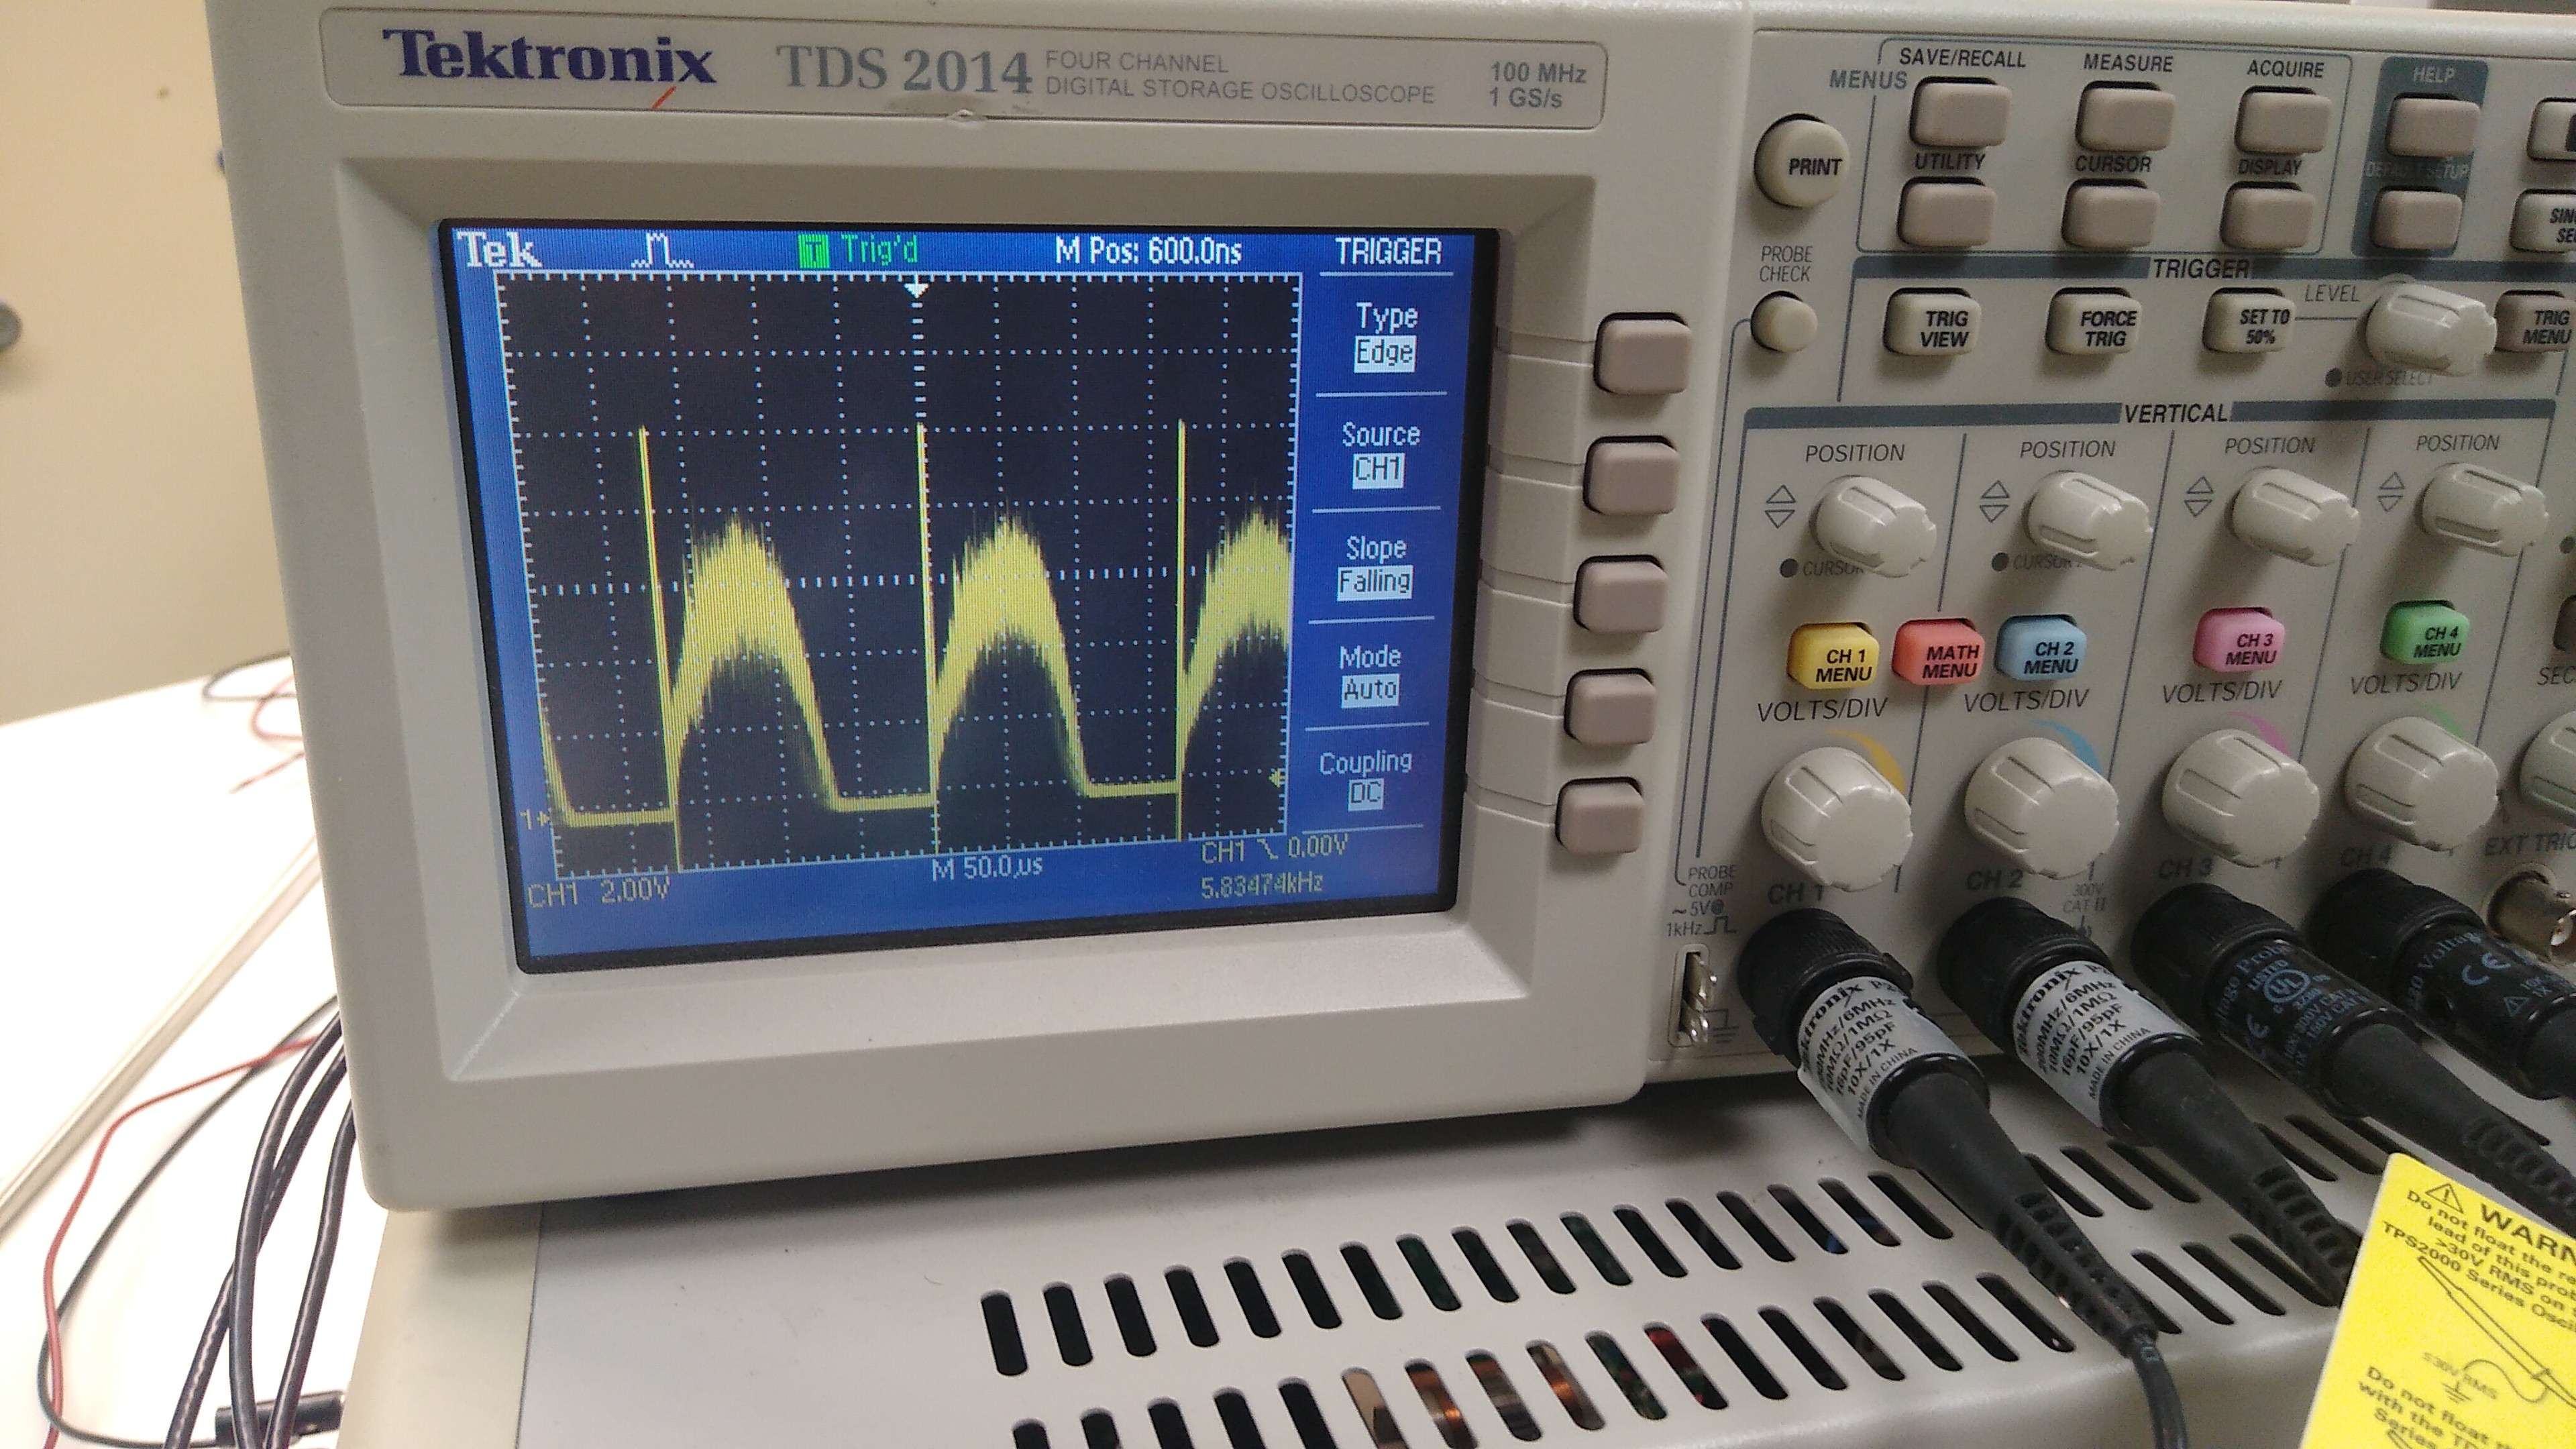
\includegraphics[width=0.5\linewidth]{Figures/PPDScopeNoise}
\end{center}
\caption{Noise after campaign with old laser.}
\label{fig:PPDScopeNoise}
\end{figure}

When an object was inserted into the optics chamber, the output resembled a square wave. This is shown in Fig. \ref{fig:PPDScatterOutput}.

\begin{figure}[H]
\begin{center}
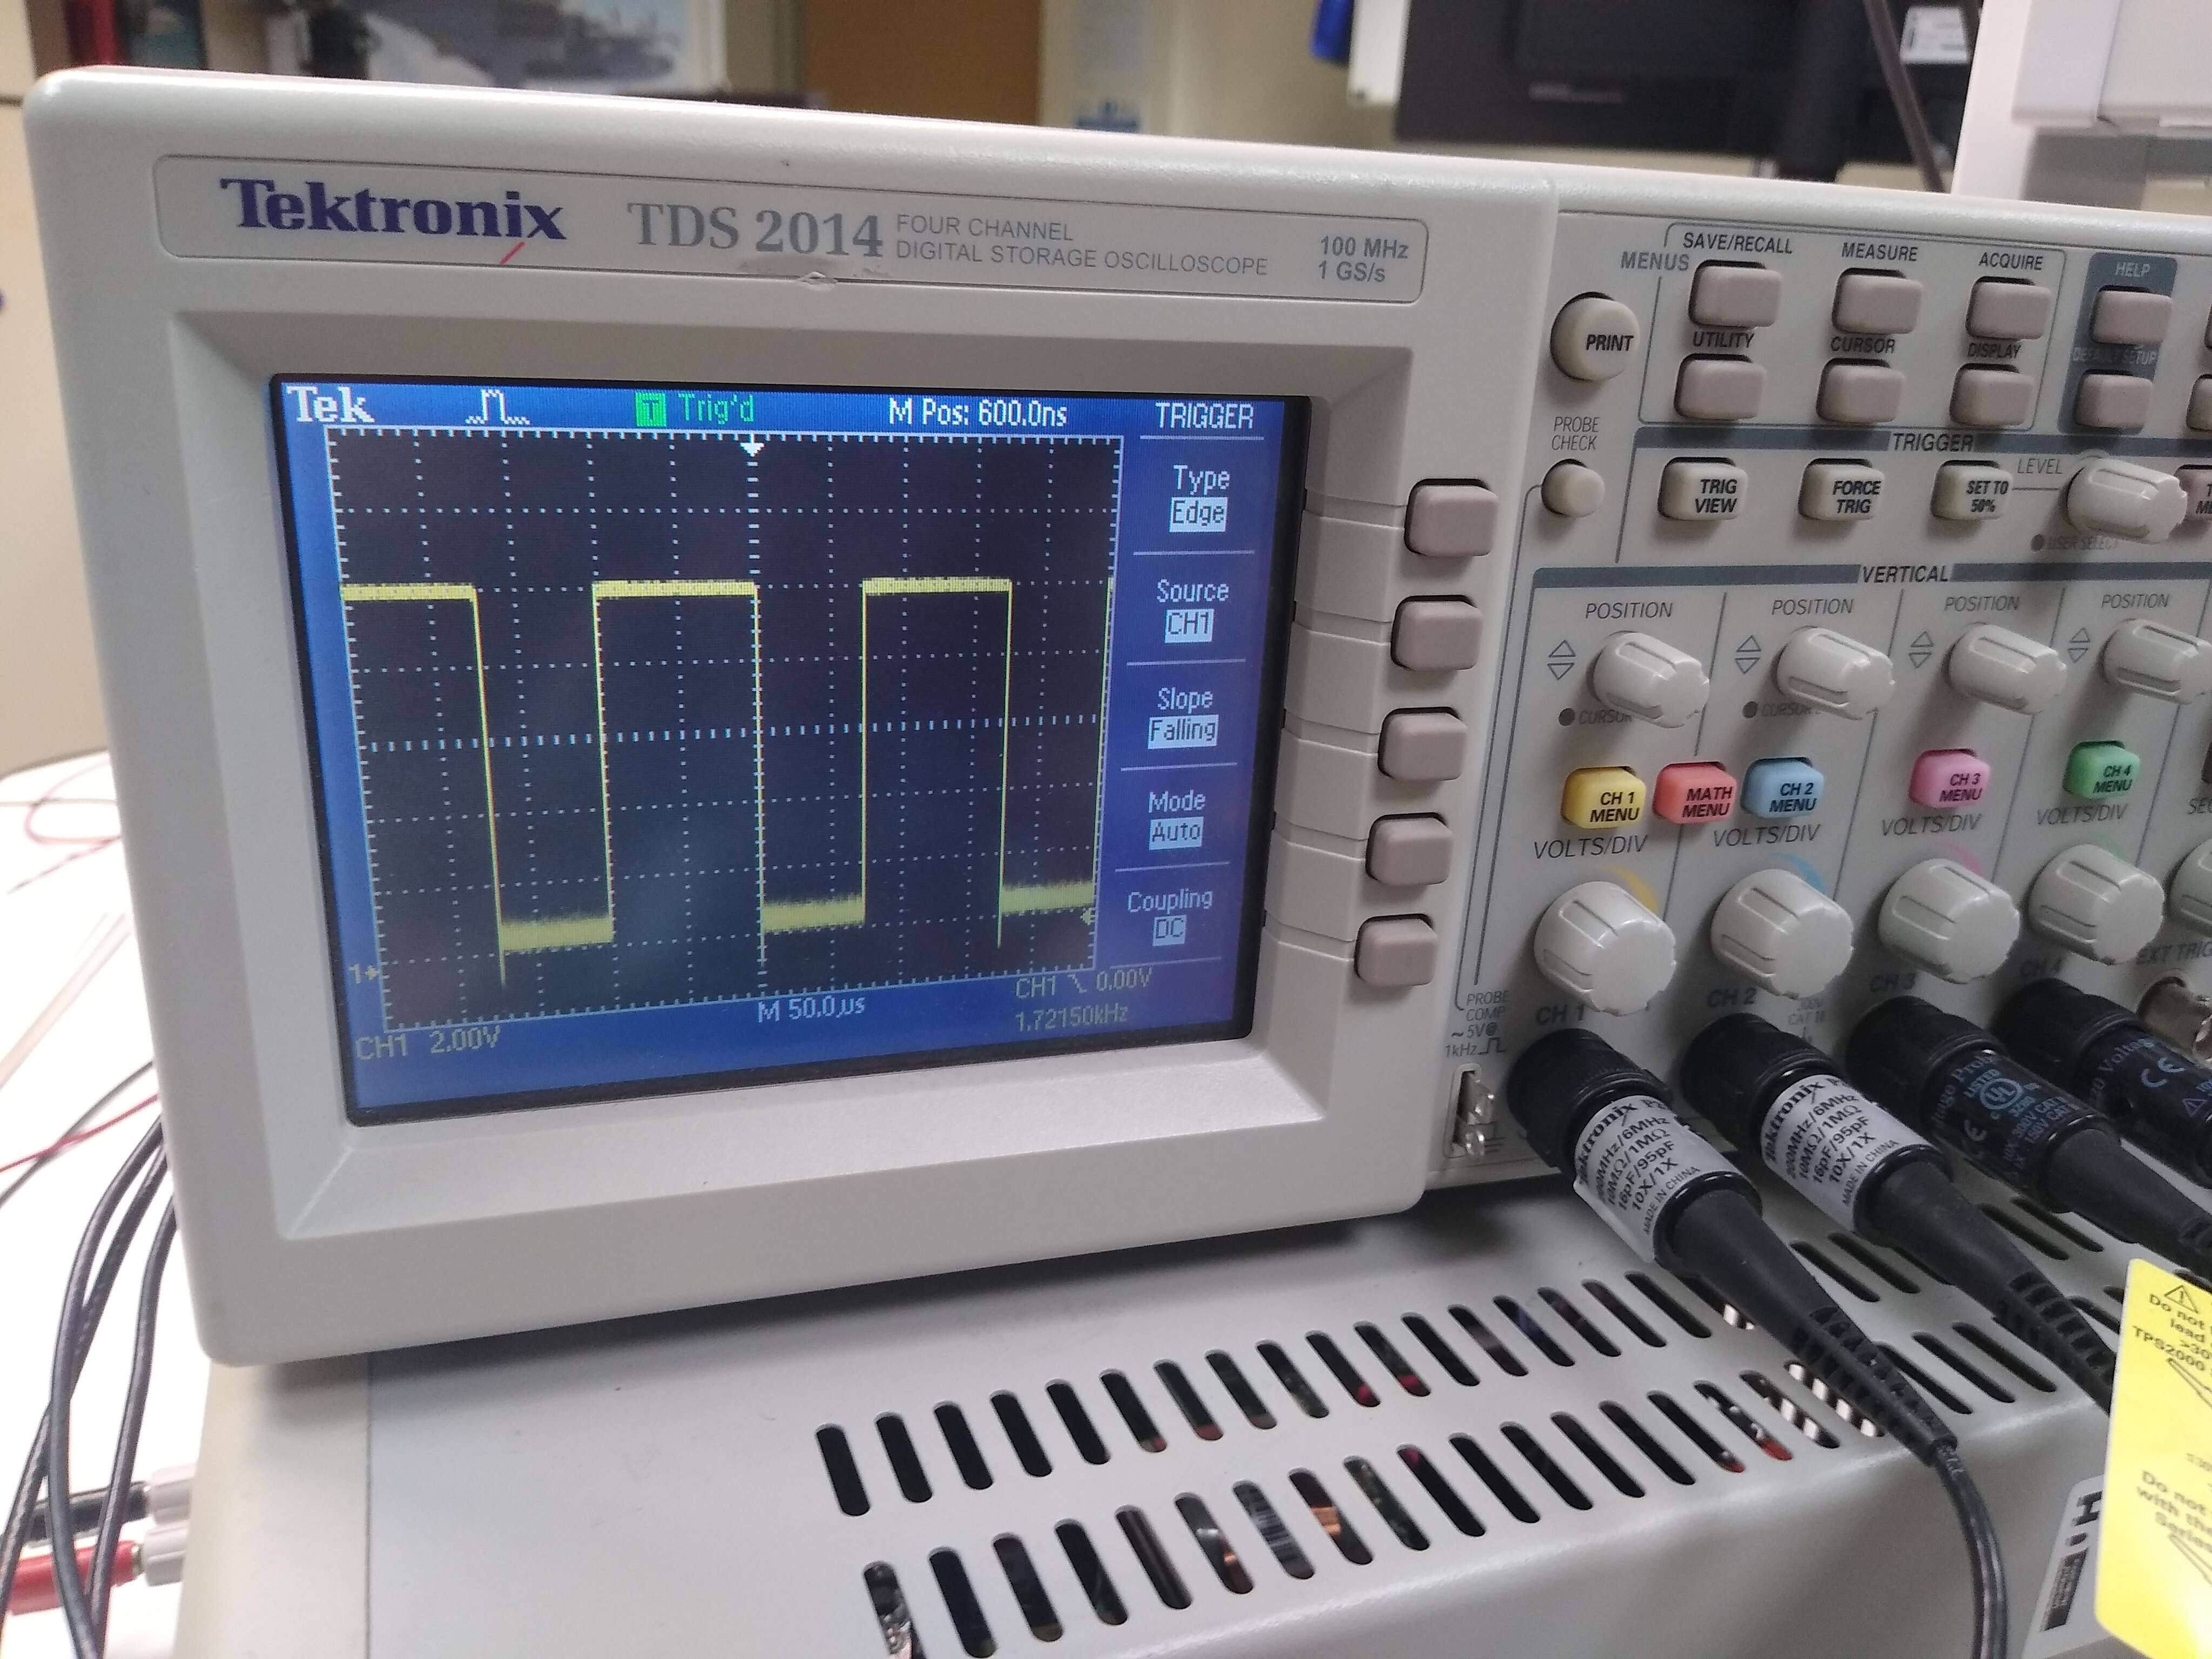
\includegraphics[width=0.5\linewidth]{Figures/PPDScatterOutput}
\end{center}
\caption{Noise after campaign with old laser and object in beam.}
\label{fig:PPDScatterOutput}
\end{figure}

The beam was also visibly dimmer, which would explain the lower image intensity. A pulse generator was configured to trigger the camera with a simulated 5 particles per second, each with a \SI{10}{\micro\second} pulse width. The camera triggering was unreliable, oftentimes exhibiting the characteristics of a "busy port".

It was decided that a new laser was the preferable option. A replacement CrystaLaser \SI{532}{\nano\metre} at \SI{150}{\milli\watt} was located.

\labday{29 March 2023}

\experiment{PPDr}

The new laser needed to be aligned since it hit the beamstop in the incorrect place, and did not pass straight through the aperture in the chamber. It was determined at a first glance that the previous alignment system would be unsuitable fo use, since it was locked in place with cyano-threadlocker. The two axes of motion couold be acheived by moving the laser on the screws, and placing shims beneath the laser to raise or lower it in one place.

It was found that the four mounting screws did not leave enough motion to rotate the laser laterally into the correct position. Two screws were removed, and the correct displacement could therefore be acheived. However, at this point, the images provided by PPD were not bright enough, and the laser was still visibly dark. An alignment tool was constructed from 3d printed PLA and a \SI{55}{\micro\metre} fibre, which could be screwed into the scattering chamber and intersect the beam. Figure \ref{fig:PPDFibreScatter} shows the scattering off the fibre, with the camera being triggered by a pulse generator, and the trigger PMT disconnected. The shape of the output seems reasonable, but the intensity of the image is very low, and the laser was visibly dim.

\begin{figure}[H]
\begin{center}
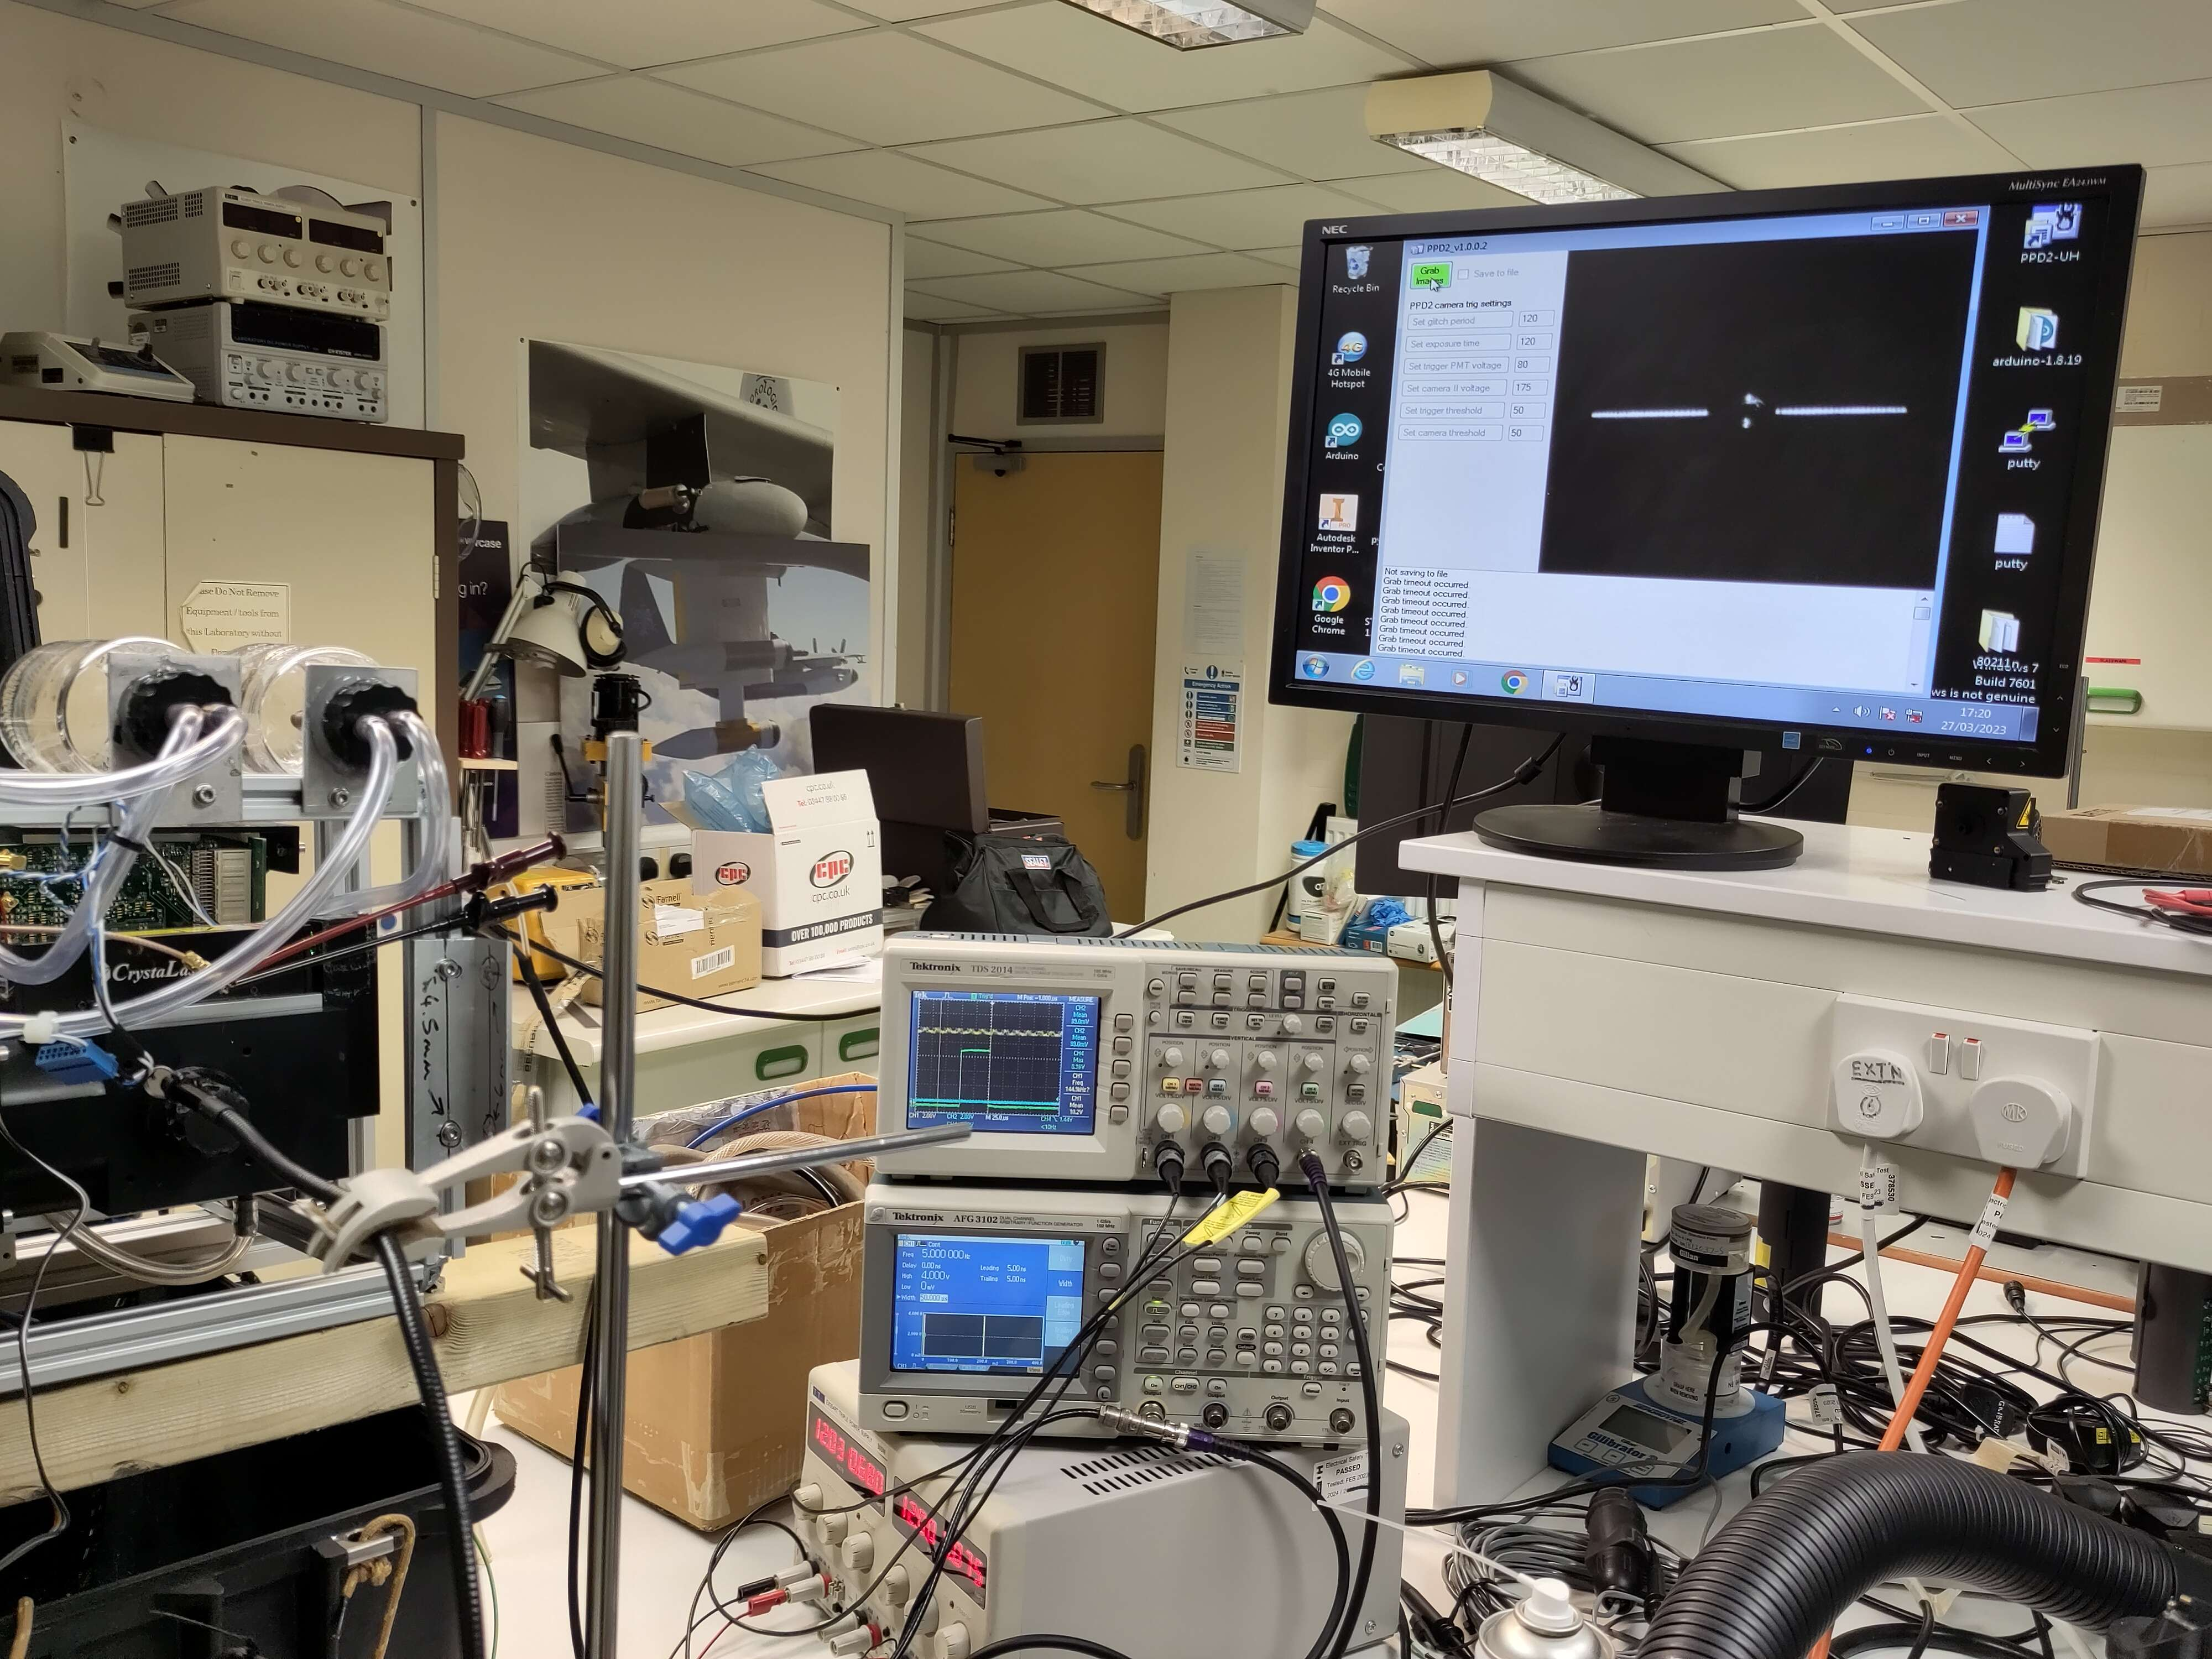
\includegraphics[width=0.5\linewidth]{Figures/PPDFibreScatter}
\end{center}
\caption{Scattering offf fibre tool.}
\label{fig:PPDFibreScatter}
\end{figure}

In order to observe the laser to further dianose issues, a beamview camera was used. The laser was reflected out of the optical block with a mirror, through an OD 2.0 neutral density filter, which lowered the output beam power to below \SI{1}{\milli\watt}, thus making it class 1. The beam appeared extremely low-quality, and looked more like diffraction off the aperture.

When the laser was tilted upwards, the beam quality improved. It was therefore determined that shims needed to be positioned beneath the front of the laser in order to acheive the desired alignment. Tilting of the laser adjusted the position of the beam relative to the aperture. It was determined through trail and improvement that two peices of paper or seven peices of foil were perfect, this is pictured in Fig. \ref{fig:PPDFoilLaser}

\begin{figure}[H]
\begin{center}
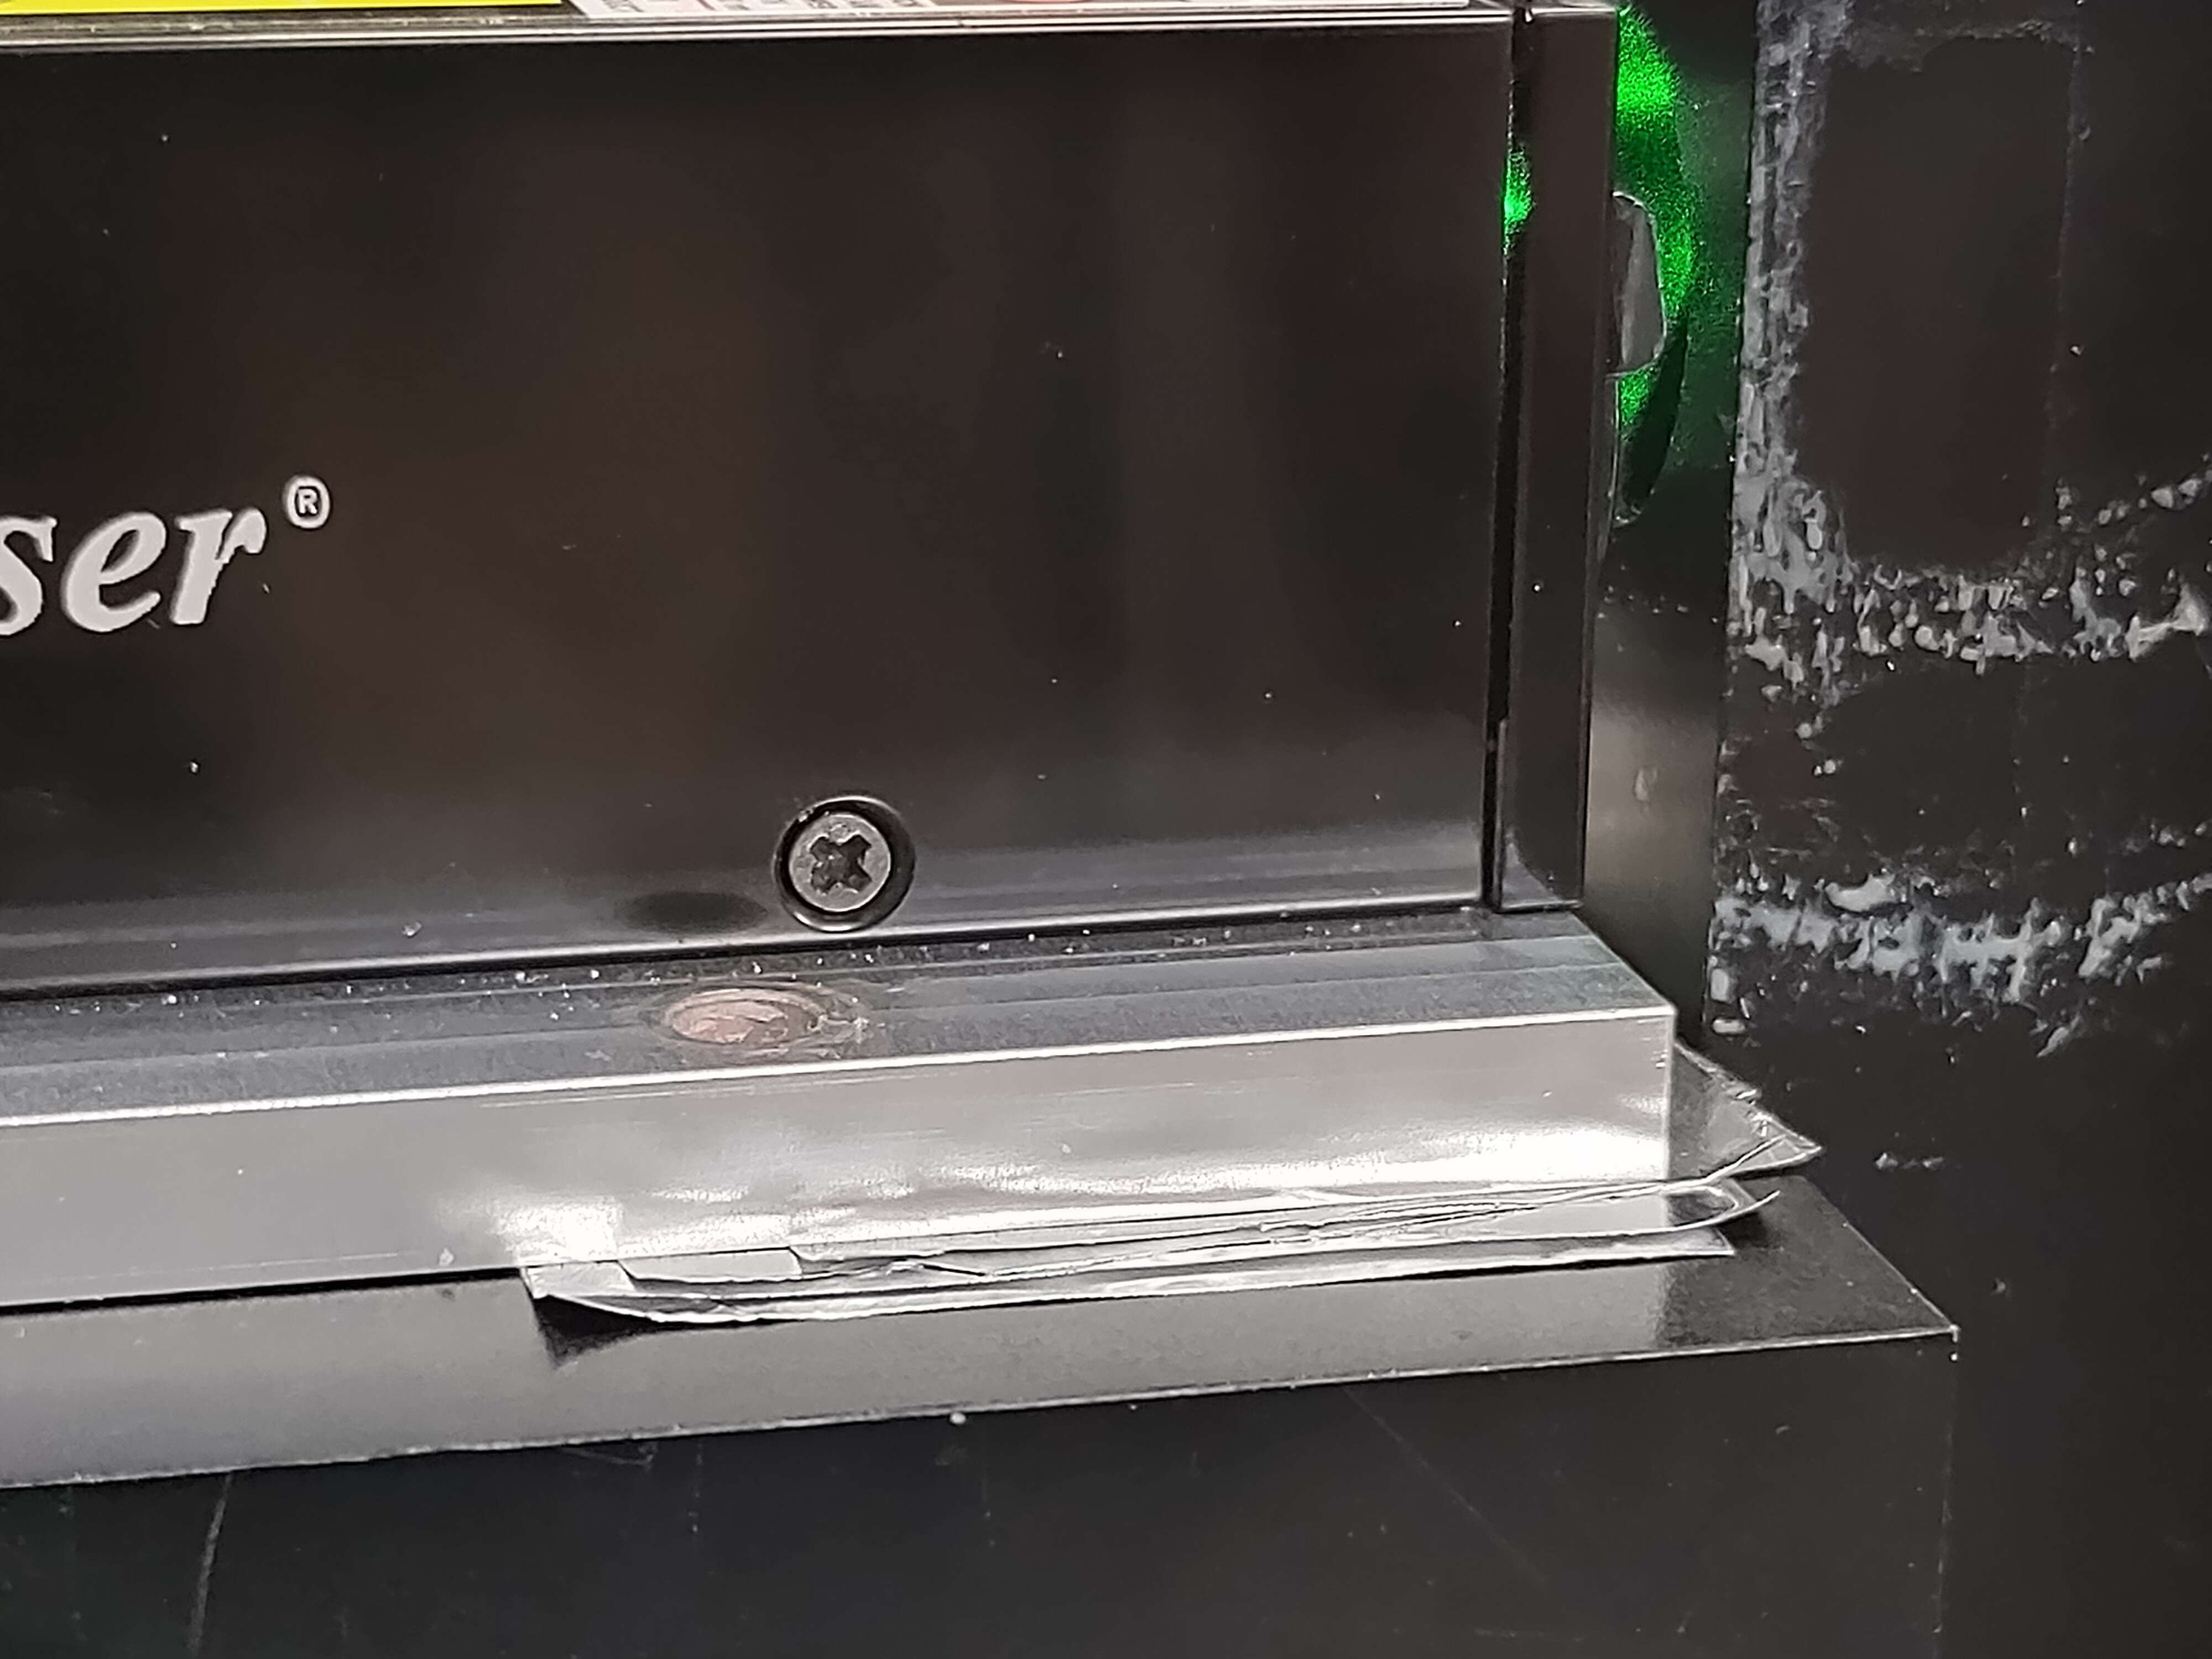
\includegraphics[width=0.5\linewidth]{Figures/PPDFoilLaser}
\end{center}
\caption{Image of foil beneath laser required for alignment.}
\label{fig:PPDFoilLaser}
\end{figure}

\labday{30 March 2023}

\experiment{PPDr}

The PPD was re-assembled for testing, the trigger PMT was re-connected. A new pump was fitted since the old one was broken by (suspected) water ingress. The flow of the pump was adjusted until \SI{6}{\litre\per\minute} was shown on the gilibrator flow-meter. Droplets were observed on the detector nicely :)

\begin{figure}[H]
\begin{center}
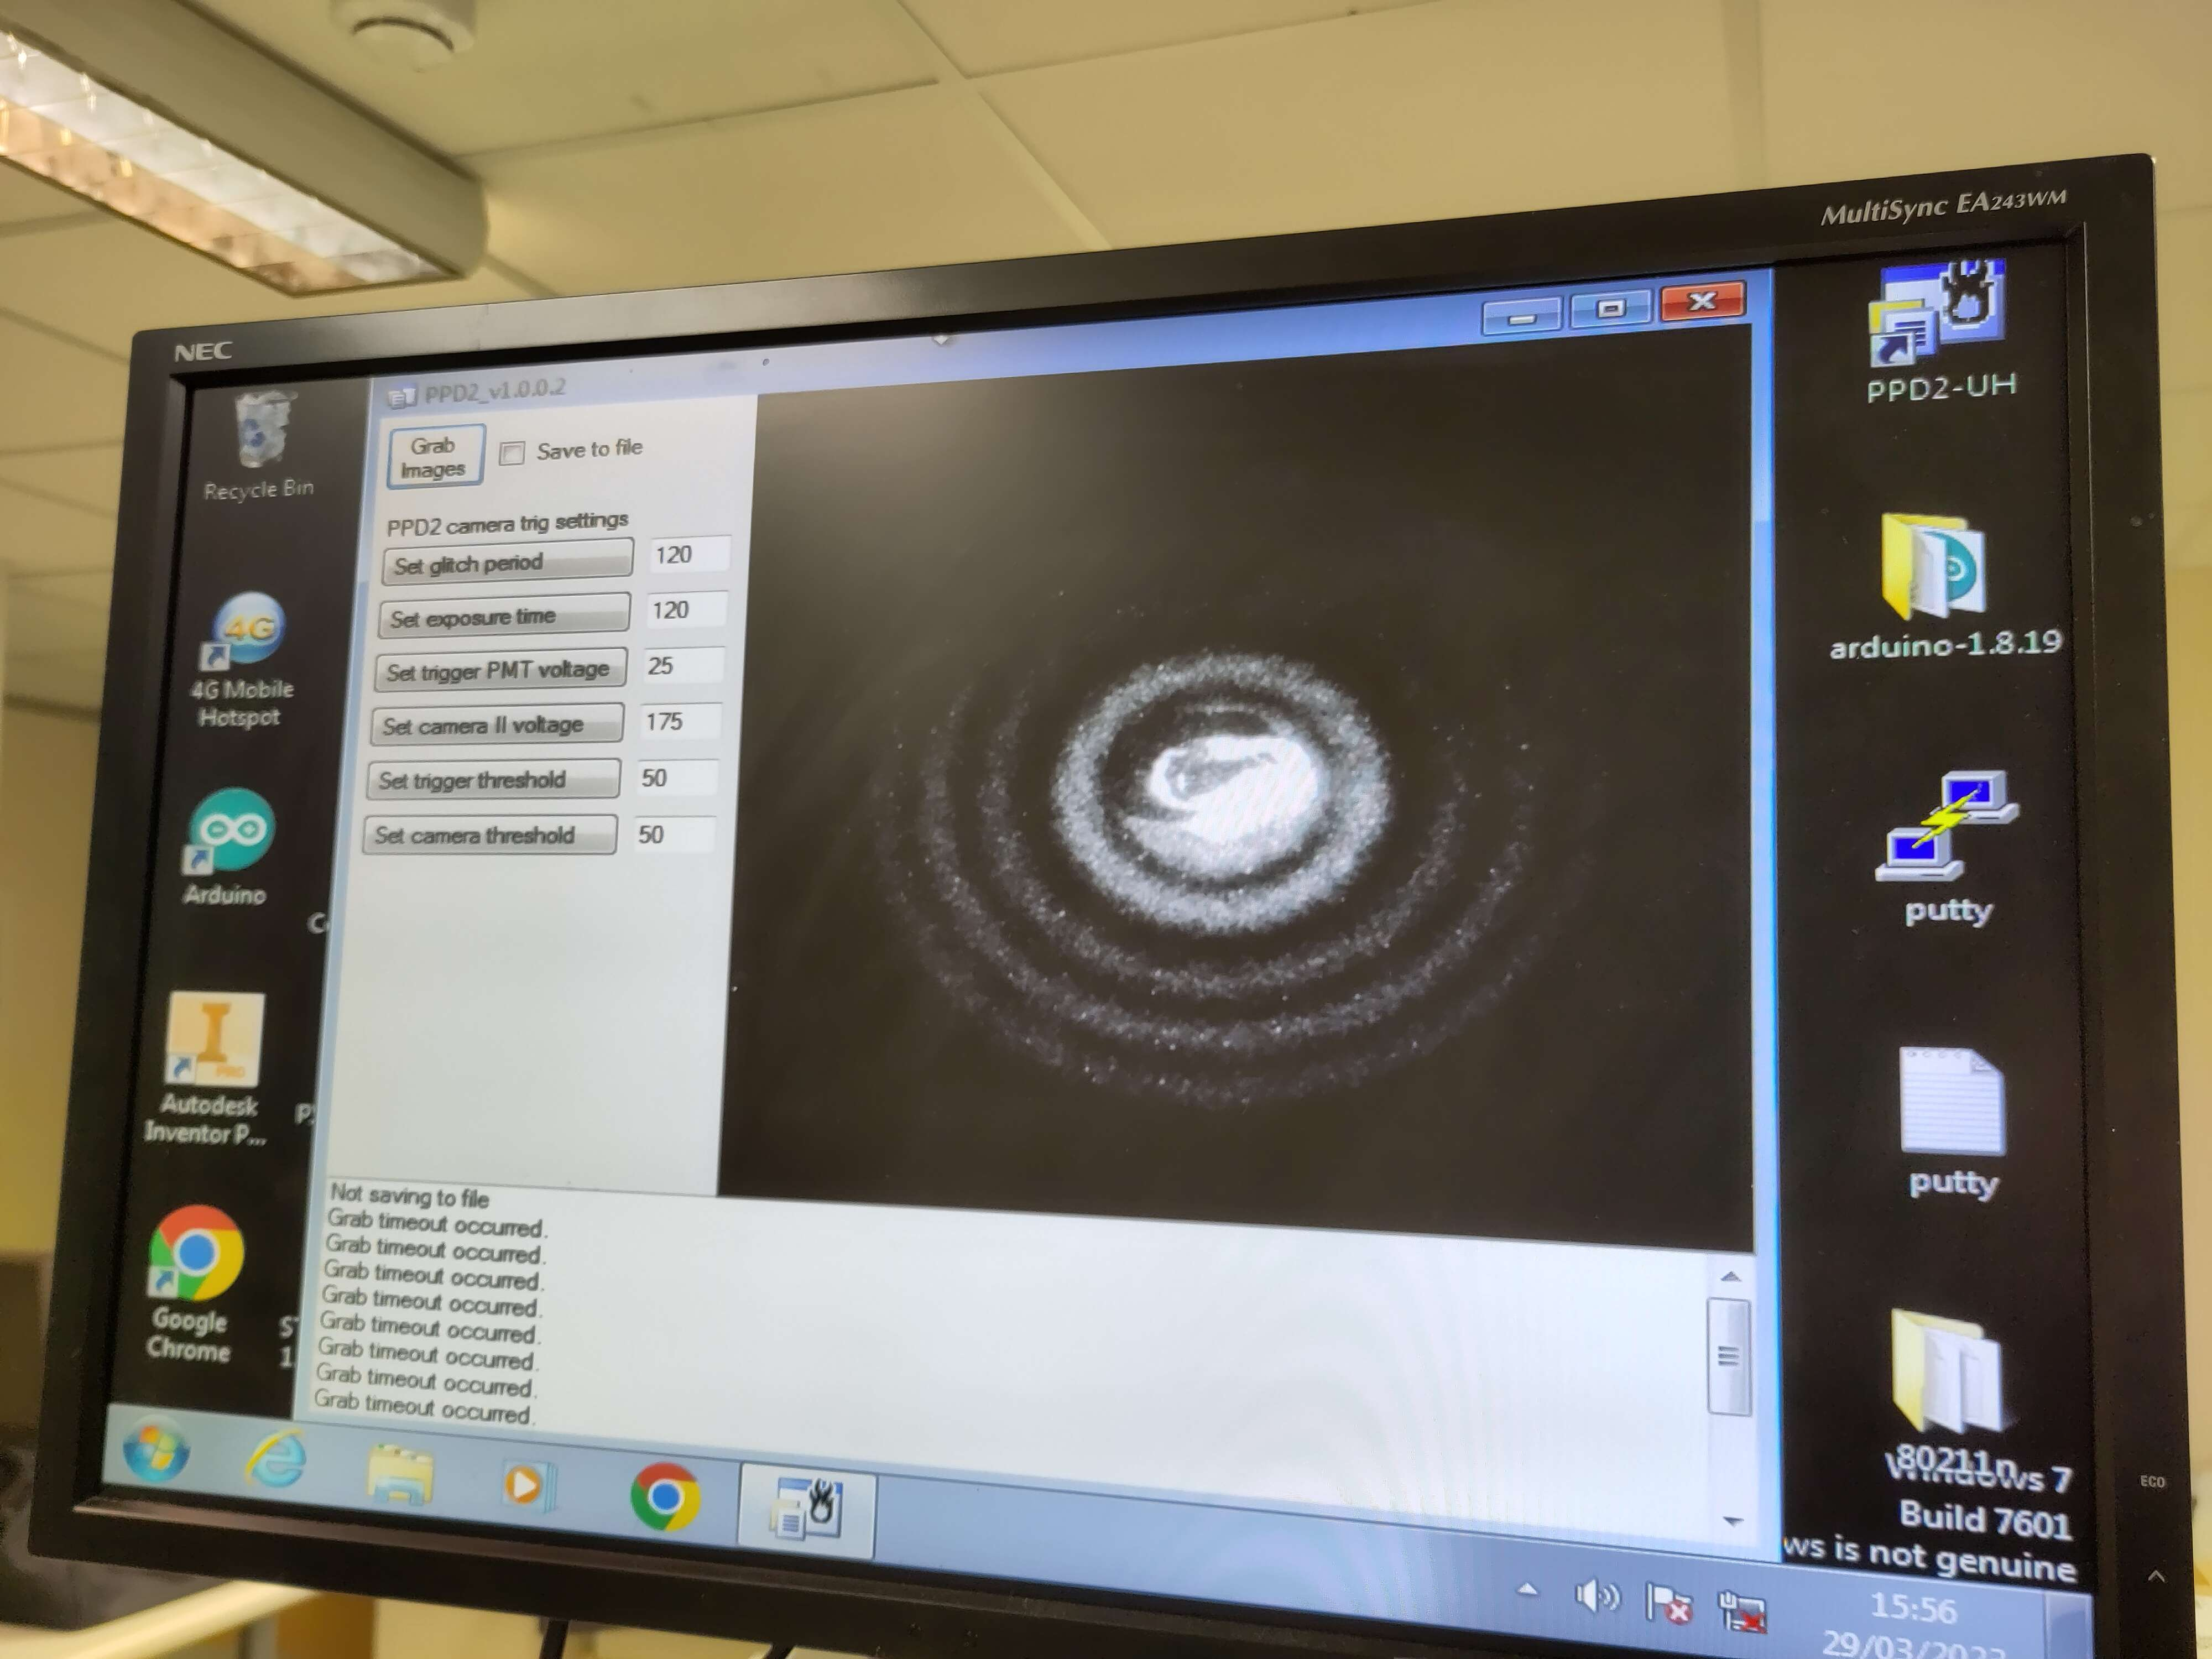
\includegraphics[width=0.5\linewidth]{Figures/PPDDropletImage}
\end{center}
\caption{Image of droplet scattering.}
\label{fig:PPDDropletImage}
\end{figure}

Ther eis still a huge problem with the computer images. There is a grab timeout which seems to randomly occur. Using a new computer with a firewire port which does not go through a PCI slot fixed the issue. It was determined that waiting for the latte-panda computer to arrive would be the preferable option for the new system. In addition, it was determined that transfering the PPD to a new case was the preferable option.


\end{document}
















